% !TeX root=../main.tex
\chapter{مشارکت در موضوع}

در ابتدا راهکارهای پیشنهادی در مقالات فصل 2 مورد بررسی قرار می‌گیرند، سپس با استفاده از آنها و در تکمیل راه‌حل‌های ارائه شده‌ی تا کنون، برای حل مسئله‌ی ذخیره‌سازی در شبکه‌ی اینترنت وسایل نقلیه استراتژی ذخیره‌سازی جدید و قابل قبولی ارائه می‌گردد. 
%\thispagestyle{empty} 

\section{نقدی بر مقالات فصل 2}
به طور کلی در هر دامنه‌ی تعریفی بزرگترین مشکلی که ‌یادگیری تقویتی عمیق با آن مواجه است، پایین بودن سرعت همگرایی به مقدار بهینه می‌باشد به علاوه‌ی اینکه تعامل با محیط برای تخمین میزان محبوبیت فایل‌ها هزینه دارد. جدای از این موارد، استفاده‌ی از شبکه‌ی عصبی باعث همگرایی به نقاط بهینه‌ی محلی می‌شود که با استفاده از تکنینک‌هایی می‌توان نقاط همگرایی را بهبود بخشید. به عنوان مثال در مقاله‌ی \cite{wu2021caching} با استفاده از الگوریتم \lr{Bootstrapped DQN} به جای \lr{Double DQN} یا \lr{DQN}، می توان متوسط پاداش‌های دریافتی را با واریانس کمتری تخمین زد. 

در واقع در الگوریتم \lr{Bootstrapped DQN} از چندین شبکه‌ی عصبی برای تخمین ارزش استیت-اکشن‌ها و یک بافر تجربیات استفاده می‌شود. برای تخمین ارزش استیت-اکشن‌ها، تجربیات تا این لحظه به عنوان ورودی بین شبکه‌های عصبی تقسیم می‌شود و خروجی‌های مربوط به آن از طریق یک شبکه‌ی مشترک بین شبکه‌های عصبی ارزیابی شده و به این ترتیب ارزش استیت-اکشن‌ها به مقادیر محلی بهینه‌تری همگرا می‌شود. در شکل \ref{fig:bootstrappeddqn} که برگرفته از مقاله‌ی \cite{osband2016deep} می‌باشد، دیاگرام مربوط به این الگوریتم را مشاهده می‌کنید.

\begin{figure}[ht]
	\centerline{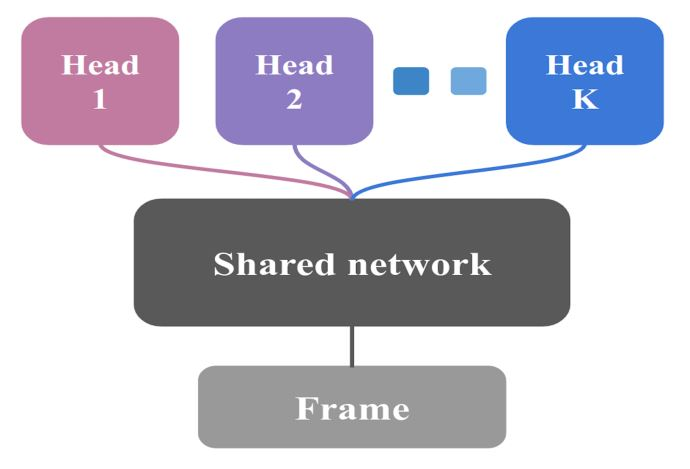
\includegraphics[width=6cm]{bootdqn}}
	\caption{دیاگرام الگوریتم \lr{Bootstrapped DQN}}
	\label{fig:bootstrappeddqn}
\end{figure}

\newpage
استفاده از خوشه‌بندی مطابق با آنچه که در مقاله‌ی \cite{majidi2021hfdrl} آورده شده است یا با استفاده از معماری ریشه-برگ در مقاله‌ی \cite{wu2022deep} با توجه به توپولوژی شبکه، می‌تواند تنوع محتویات کش شده در حافظه‌ی گره‌های لبه را در محیط‌های تعاملی چندعامله افزایش دهد و بنابراین میزان موفقیت حافظه‌ی کش در تأمین دیتای درخواستی نیز افزایش می‌یابد. البته در این مقالات درباره‌ی نحوه‌ی آپدیت خوشه‌بندی‌های موجود صحبتی به میان نیامده حال آنکه یکی از ویژگی‌هایی که در خوشه‌بندی لحاظ می‌شود الگوی درخواستی کاربران است و با توجه به غیرایستان بودن محیط، این الگو با زمان تغییر می‌یابد و لازم است تا خوشه‌بندی‌ها نیز آپدیت شوند که در بخش بعدی راه حلی برای رویارویی با این چالش ارائه می‌شود.

\section{بیان مشارکت}
طبیعت محیط در انتخاب الگوریتم یادگیری تقویتی مناسب برای تخمین میزان محبوبیت فایل‌ها تأثیر به سزایی دارد. به عنوان مثال در مقاله‌ی \cite{qiao2019deep} دیدیم که در نظر گرفتن حرکت گره‌های مصرف کننده در شبکه‌های اینترنت اشیا، بر تعریف مجموعه‌ی استیت‌ها و اکشن‌ها اثر ‌می‌گذارد و نیز دیدیم که مقاله  روشی را برای تخمین سیاست بهینه به طور مستقیم ارائه کرده بود. حال برای شبیه‌سازی شبکه‌های اینترنت وسایل نقلیه، استفاده از سیمولاتوری مانند \lr{OMNET++} برای شبیه‌سازی شبکه‌ی هدف و عامل‌های به کار رفته در محیط، می‌تواند راهگشا باشد.

علاوه بر این برای حل مشکل سرعت همگرایی استفاده از الگوریتم \lr{Penalized NFAC (PeNFAC)} که در مقاله‌ی  \cite{zimmer2019exploiting} معرفی شده است به جای  \lr{DDPG}، می‌تواند به ما در تخمین مستقیم سیاست بهینه کمک کند. در مقاله‌ی \cite{zimmer2019exploiting} کارکرد دو الگوریتم نامبرده با یکدیگر مقایسه شده است و دیده می‌شود که سرعت همگرایی \lr{PeNFAC} نسبت به \lr{DDPG} به سیاست بهینه بیشتر بوده و در ضمن مجموع پاداش‌های دریافتی در \lr{PeNFAC} نسبت به \lr{DDPG} به مقدار بیشتری همگرا می‌گردد و از الگوریتم \lr{PeNFAC} در حالت‌های کنترلی متمرکز و غیرمتمرکز می‌توان استفاده نمود.

در ادامه برای آپدیت خوشه بندی‌های مبتنی بر الگوریتم \lr{K-means} در استراتژی ذخیره سازی چندعامله در محیط شبکه‌های اینترنت وسایل نقلیه، از متدهای مربوط به \lr{Transfer Learning} می‌توان استفاده کرد. در واقع در این دسته از متدها از دانسته‌های قبلی برای آپدیت مدل برای تسک جدید (که در اینجا هایپر پارامتر \lr{K} با توجه به شرایط جدید محیطی آپدیت می‌شود.) استفاده می‌شود. 

در مسئله‌ی بهینه سازی مطرح شده، تابع هدف ما کاهش تابع هزینه‌ی وزندار حاصل از سه پارامتر مصرف انرژی در حسگرها، طول عمر دیتا (مدت زمانی که از اعتبار دیتا گذشته) و ترافیک لینک های پشتی می‌باشد.
